
\section{MET Templates}
\label{sec:templates}

The premise of this data driven technique is that MET in \Z plus jets events
is produced by the hadronic recoil system and {\it not} by the leptons making up the \Z.
Therefore, the basic idea of the MET template method is to measure the MET distribution in 
a control sample which has no true MET and the same general attributes regarding
fake MET as in \Z plus jets events.
In our case, we choose a photon-like sample. These are not necessarily photons, but jets with predominantly 
electromagnetic energy deposition in a good fiducial volume. This ensures that 
they are well measured and do not contribute to fake MET.

Both the control sample and the \Z plus jets background
consist of a well measured object (either a photon or a leptonically decaying \Z), which recoils 
against a system of hadronic jets. The MET in these events 
is then dominated by mismeasurements of the hadronic system. To account for kinematic 
differences between the hadronic systems in the control vs. signal samples, 
we measure the MET distributions in the control sample in bins of the number of jets and the 
scalar sum of jet \pt. In order to track conditions which change over the course of data-taking
(most notably the increased pile-up) and to increase the statistics at large photon \pt, we
use multiple photon triggers ``stitched'' together. Each photon event enters the template for the
highest \pt photon trigger which fired in the event. The resulting MET 
distributions in each bin of njets, sumjetpt and photon trigger are then normalized to unit area, yielding an array of MET templates. 
Each \Z event is then assigned one such 
unit area template based on its number of jets, the scalar sum of jet \pt and the Z \pt.
%{\bf Claudio: currently the Z pt is used to determine which trigger template set to use. You argued earlier that instead
%\bf we should use the pt of the hadronic recoil. I have verified that this makes a negligible difference, but if you prefer,
%\bf I can switch to using hadronic recoil pt.} 
The sum of these templates for all selected \Z events then forms the 
prediction of the MET distribution for the \Z sample. Integrating this prediction for our 
signal regions  thus provides a data driven prediction for the \Z plus jets yields in the signal regions. 


The MET templates are derived from a set of photon triggered samples. 
The Njet binning used is 2 jets and $\ge$ 3 jets. 
The sum jet \pt binning is defined by the boundaries {0, 30, 60, 90, 120, 150, 250, 5000}~GeV.
The photon triggers, and the ranges of \Z \pt for which they are selected, are (the triggers with ``v1'' in their name appear in later runs):

\begin{itemize}
\item \verb=HLT_Photon20_Cleaned_L1R= (\Z \pt $<$ 32~GeV)
\item \verb=HLT_Photon30_Cleaned_L1R= (32 GeV $<$ \Z \pt $<$ 52~GeV)
\item \verb=HLT_Photon50_Cleaned_L1R= (52 GeV $<$ \Z \pt $<$ 72~GeV)
\item \verb=HLT_Photon50_Cleaned_L1R_v1= (52 GeV $<$ \Z \pt $<$ 72~GeV)
\item \verb=HLT_Photon70_Cleaned_L1R_v1= (\Z \pt $>$ 72~GeV)
\end{itemize}

We show all the templates used in App.~\ref{sec:appendix_templates}.

%The prediction is then formed by selecting the photon trigger based on the \pt of the \Z in the event which is being predicted
%\begin{figure}[h]
%  \begin{center}
%    \resizebox{0.75\linewidth}{!}{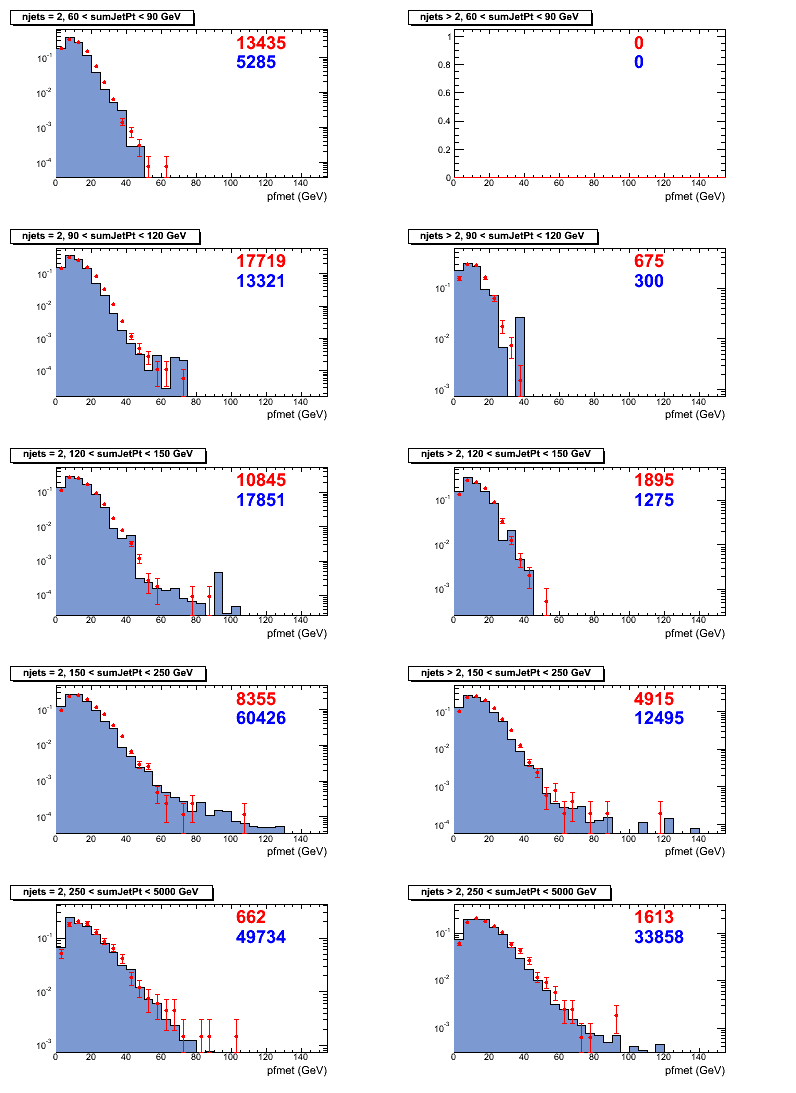
\includegraphics{plots/alltemplates.png}}
%    \caption{    \label{fig:templates} The templates for pfMET in Njet = 2 (left column), and Njet $\ge$ 3 (right column) in the sum jet \pt ranges printed on the plots.
%      PhotonJet MC is indicated by the solid histogram, data is indicated by the points with error bars. The number of entries in each bin 
%      are shown for MC (blue) and data (red).}
%  \end{center}
%\end{figure}

%In order to select a photon sample whose \pt distribution matches the distribution of \Z \pt
% in our preselection, a combination of photon triggers must be used (see below). 
%In order to account for varying prescales of the triggers in different runs,
% separate templates are created for each trigger line. 
%Each event enters the template for the highest \pt trigger which fires in the event,
% and the template is filled with a weight equal to the prescale of the corresponding trigger.
%After this procedure, the templates are normalized to unity.